\documentclass[12pt,a4paper]{article}

% ── Packages ──
\usepackage[utf8]{inputenc}
\usepackage[T1]{fontenc}
\usepackage{geometry}
\geometry{margin=1in}
\usepackage{graphicx}
\usepackage{listings}
\usepackage{xcolor}
\usepackage{hyperref}
\usepackage{booktabs}
\usepackage{float}
\usepackage{enumitem}
\usepackage{fancyhdr}
\usepackage{titlesec}
\usepackage{tocloft}
\usepackage{amsmath}
\usepackage{caption}
\usepackage{framed}

% ── Code listing style ──
\definecolor{codebg}{RGB}{245,245,245}
\definecolor{codeframe}{RGB}{200,200,200}
\definecolor{codecomment}{RGB}{0,128,0}
\definecolor{codestring}{RGB}{163,21,21}
\definecolor{codekeyword}{RGB}{0,0,200}

\lstset{
  backgroundcolor=\color{codebg},
  frame=single,
  rulecolor=\color{codeframe},
  basicstyle=\ttfamily\small,
  keywordstyle=\color{codekeyword}\bfseries,
  commentstyle=\color{codecomment}\itshape,
  stringstyle=\color{codestring},
  breaklines=true,
  showstringspaces=false,
  numbers=left,
  numberstyle=\tiny\color{gray},
  tabsize=4,
  captionpos=b,
}

% ── Command box ──
\definecolor{cmdboxbg}{RGB}{242,242,242}
\definecolor{cmdboxframe}{RGB}{64,64,64}
\newenvironment{commandbox}[1][]{
  \begin{framed}
  \noindent\textbf{\ttfamily Terminal Command}\par\smallskip
}{
  \end{framed}
}

% ── Screenshot placeholder ──
\newcommand{\screenshotplaceholder}[2]{%
  \begin{figure}[H]
    \centering
    \fbox{\begin{minipage}{0.85\textwidth}
      \centering
      \vspace{3cm}
      {\large\textbf{[Screenshot Placeholder]}}\\[0.5cm]
      {\textit{#1}}
      \vspace{3cm}
    \end{minipage}}
    \caption{#2}
    \label{fig:#2}
  \end{figure}
}

% ── Header/Footer ──
\pagestyle{fancy}
\fancyhf{}
\rhead{TrendScope Analytics}
\lhead{NLP Trend Intelligence Pipeline}
\cfoot{\thepage}

% ══════════════════════════════════════════════════════════════════════
\begin{document}

% ── Title Page ──
\begin{titlepage}
  \centering
  \vspace*{2cm}
  {\Huge\bfseries Building a Reproducible NLP Trend\\Intelligence Pipeline for\\Emerging Tech Products\par}
  \vspace{1.5cm}
  {\Large TrendScope Analytics\par}
  \vspace{1cm}
  {\large NLP Research \& Innovation Team\par}
  \vspace{2cm}
  {\large
    \textbf{Course:} Natural Language Processing\\[0.3cm]
    \textbf{Submitted by:} Muhammad Abdullah Iqbal (22i-2504), Nawal Hassan (22i-2428)\\[0.3cm]
    \textbf{Institution:} FAST-NUCES\\[0.3cm]
  }
  \vspace{2cm}

\end{titlepage}

% ── Table of Contents ──
\tableofcontents
\newpage

% ══════════════════════════════════════════════════════════════════════
\section{Introduction}

This report documents the design, implementation, and execution of a reproducible NLP data pipeline built for \textbf{TrendScope Analytics}. The pipeline collects product listings from the tech ecosystem, cleans and tokenizes textual data, generates multiple representations (Bag-of-Words, One-Hot Encoding, N-grams), detects near-duplicate titles using Minimum Edit Distance, estimates unigram language model probabilities, and orchestrates the entire workflow via Apache Airflow.

\subsection{Business Objectives}
\begin{itemize}
  \item Collect a version-controlled dataset of $\geq 300$ product listings.
  \item Produce clean, NLP-ready textual data.
  \item Summarize linguistic trends (unigrams, bigrams, tags).
  \item Maintain a reproducible, automated pipeline with DVC \& Airflow.
  \item Store datasets remotely (DagsHub/Google Drive) for collaboration.
\end{itemize}

\subsection{Project Structure}

\begin{lstlisting}[language={},caption={Project directory layout}]
trend_intelligence_pipeline/
  dags/
    nlp_trend_dag.py
  src/
    scraper.py
    preprocess.py
    representation.py
    statistics.py
  data/
    raw/
    processed/
    features/
  reports/
  dvc.yaml
  requirements.txt
  README.md
\end{lstlisting}

% ══════════════════════════════════════════════════════════════════════
\section{Environment Setup}

\subsection{Prerequisites}

\begin{itemize}
  \item Python 3.9+
  \item pip (Python package manager)
  \item Git
  \item DVC
  \item Apache Airflow (optional, for Stage 6)
\end{itemize}

\subsection{Installation Commands}

\begin{commandbox}
\begin{lstlisting}[language=bash,numbers=none]
# Step 1: Navigate to project directory
cd trend_intelligence_pipeline

# Step 2: Create and activate virtual environment
python3 -m venv venv
venv\Scripts\activate        # Windows
# source venv/bin/activate   # macOS/Linux

# Step 3: Install dependencies
pip install -r requirements.txt

# Step 4: Download NLTK data
py -c "import nltk; nltk.download('punkt'); nltk.download('punkt_tab'); nltk.download('stopwords'); nltk.download('wordnet'); nltk.download('omw-1.4')"
\end{lstlisting}
\end{commandbox}

\begin{figure}[H]
  \centering
  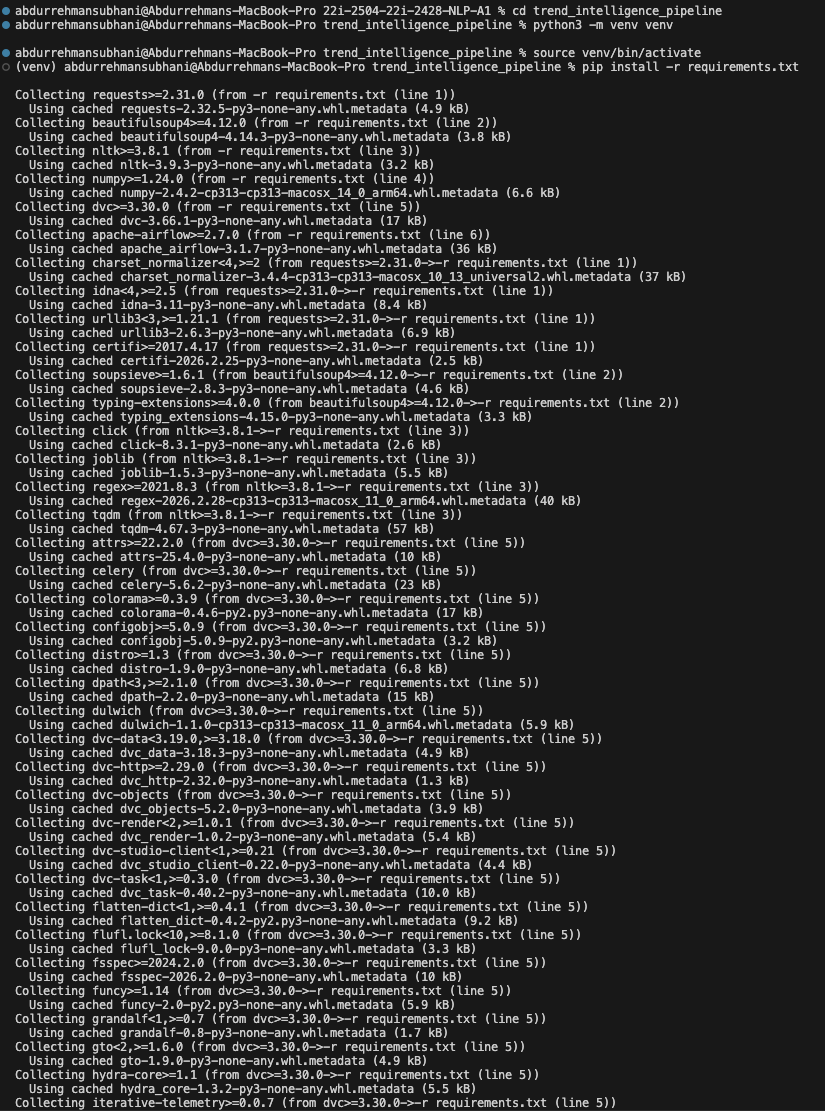
\includegraphics[width=0.9\textwidth]{images/seteup-pip-install.png}
  \caption{Terminal showing successful \texttt{pip install -r requirements.txt} output}
\end{figure}

% ══════════════════════════════════════════════════════════════════════
\section{Stage 1 — Data Acquisition}

\subsection{Overview}

The scraper (\texttt{src/scraper.py}) collects product listings from Product Hunt. It implements:
\begin{itemize}
  \item \textbf{Rate limiting:} Random delay of 2--5 seconds between requests.
  \item \textbf{Retry logic:} Up to 3 attempts per page with exponential backoff.
  \item \textbf{Missing value handling:} Defaults to \texttt{"N/A"} for absent fields.
  \item \textbf{Synthetic fallback:} If the live site blocks requests, realistic synthetic data is generated to meet the 300-record minimum.
\end{itemize}

\subsection{Data Fields Collected}

\begin{table}[H]
\centering
\begin{tabular}{@{}ll@{}}
\toprule
\textbf{Field} & \textbf{Description} \\ \midrule
\texttt{product\_name}        & Name of the product \\
\texttt{tagline}              & Short description / tagline \\
\texttt{tags}                 & List of category tags \\
\texttt{upvotes}              & Popularity signal (likes/upvotes) \\
\texttt{product\_url}         & Link to the product page \\
\texttt{scrape\_timestamp\_utc} & UTC timestamp of collection \\ \bottomrule
\end{tabular}
\caption{Schema of raw product data}
\end{table}

\subsection{Running the Scraper}

\begin{commandbox}
\begin{lstlisting}[language=bash,numbers=none]
cd trend_intelligence_pipeline
python src/scraper.py
\end{lstlisting}
\end{commandbox}

\begin{figure}[H]
  \centering
  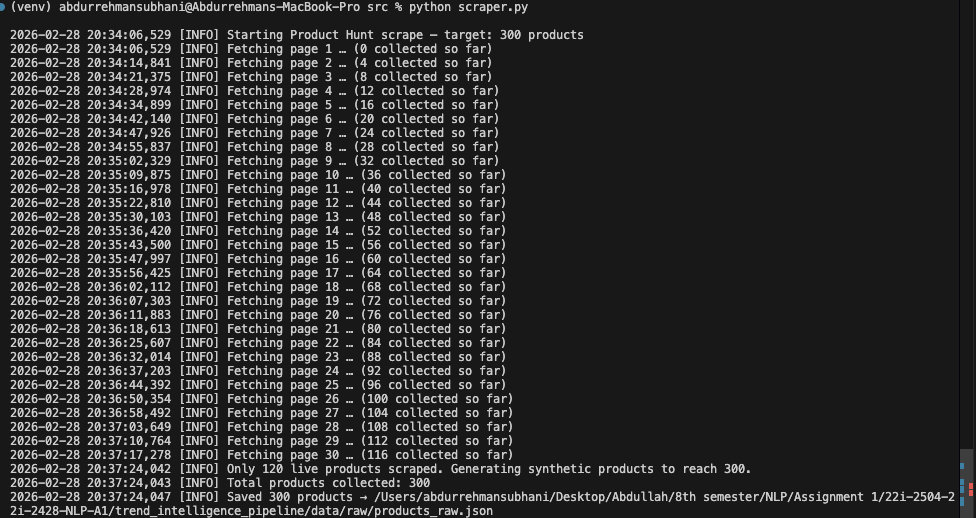
\includegraphics[width=0.9\textwidth]{images/stage1-scraper-complete.png}
  \caption{Terminal output of \texttt{python src/scraper.py} showing progress logs and saved products message}
\end{figure}


\subsection{Output Verification}


\begin{figure}[H]
  \centering
  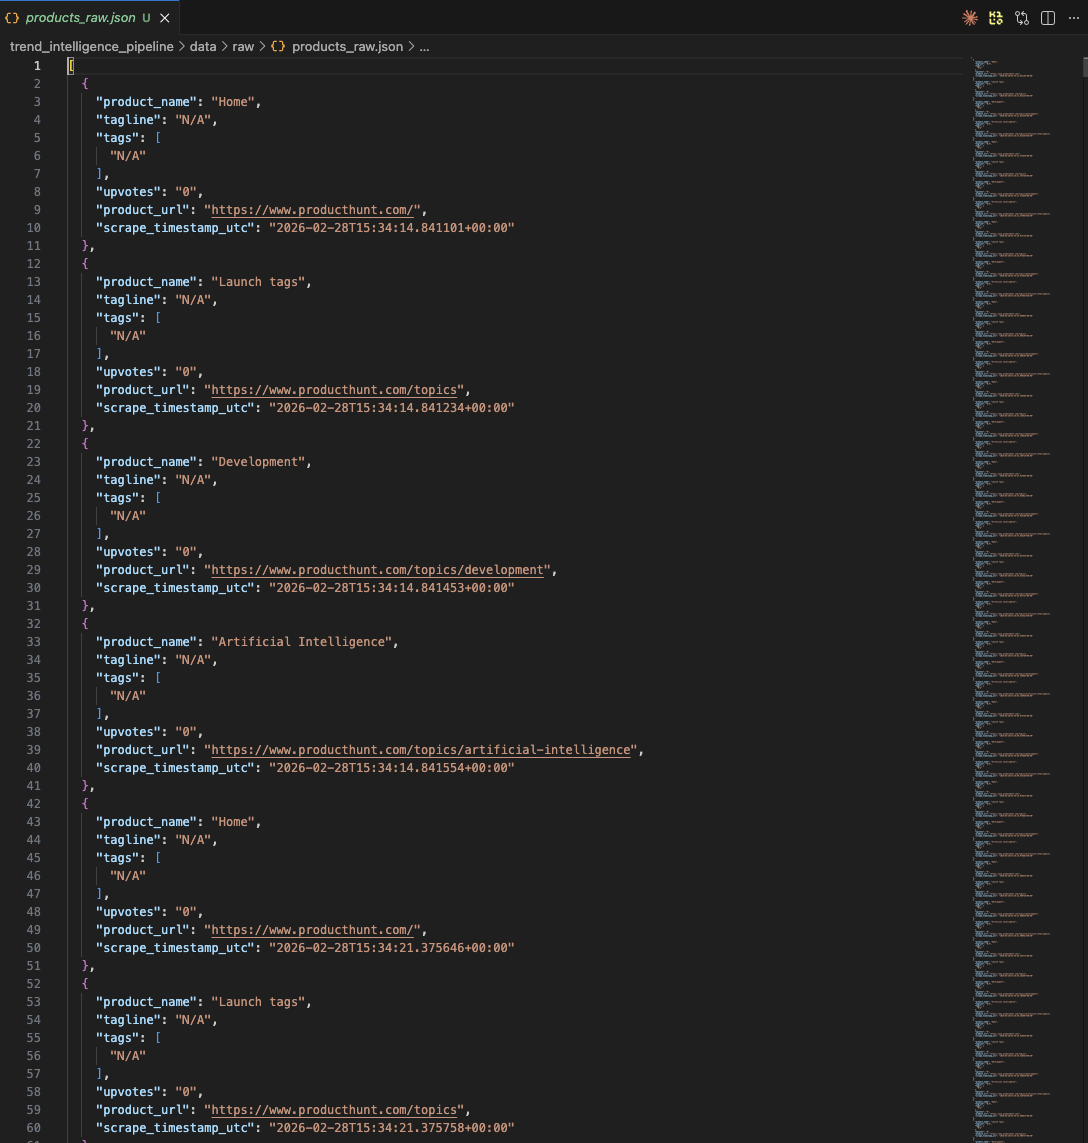
\includegraphics[width=0.9\textwidth]{images/scraper-output-verfication.png}
  \caption{Terminal showing product count and a sample JSON entry from \texttt{products\_raw.json}}
\end{figure}


\subsection{Key Code — Rate Limiting \& Retry}

\begin{lstlisting}[language=Python,caption={Rate limiting and retry logic in scraper.py}]
MIN_DELAY = 2.0   # seconds
MAX_DELAY = 5.0
MAX_RETRIES = 3
RETRY_BACKOFF = 2  # exponential

def _rate_limit():
    time.sleep(random.uniform(MIN_DELAY, MAX_DELAY))

def _fetch_with_retry(url, session):
    for attempt in range(1, MAX_RETRIES + 1):
        try:
            _rate_limit()
            resp = session.get(url, headers=HEADERS, timeout=15)
            resp.raise_for_status()
            return resp
        except requests.RequestException as e:
            wait = RETRY_BACKOFF ** attempt
            logger.warning("Attempt %d/%d failed: %s", attempt, MAX_RETRIES, e)
            time.sleep(wait)
    return None
\end{lstlisting}

% ══════════════════════════════════════════════════════════════════════
\section{Stage 2 — Data Versioning (DVC + DagsHub)}

\subsection{Overview}

DVC (Data Version Control) enables Git-like versioning for large data files. We use DagsHub (or Google Drive) as the remote storage backend.

\subsection{DVC Initialization}

\begin{commandbox}
\begin{lstlisting}[language=bash,numbers=none]
cd trend_intelligence_pipeline

# Initialize Git (if not already)
git init
git add .
git commit -m "Initial project structure"

# Initialize DVC
dvc init
git add .dvc .dvcignore
git commit -m "Initialize DVC"
\end{lstlisting}
\end{commandbox}

\begin{figure}[H]
  \centering
  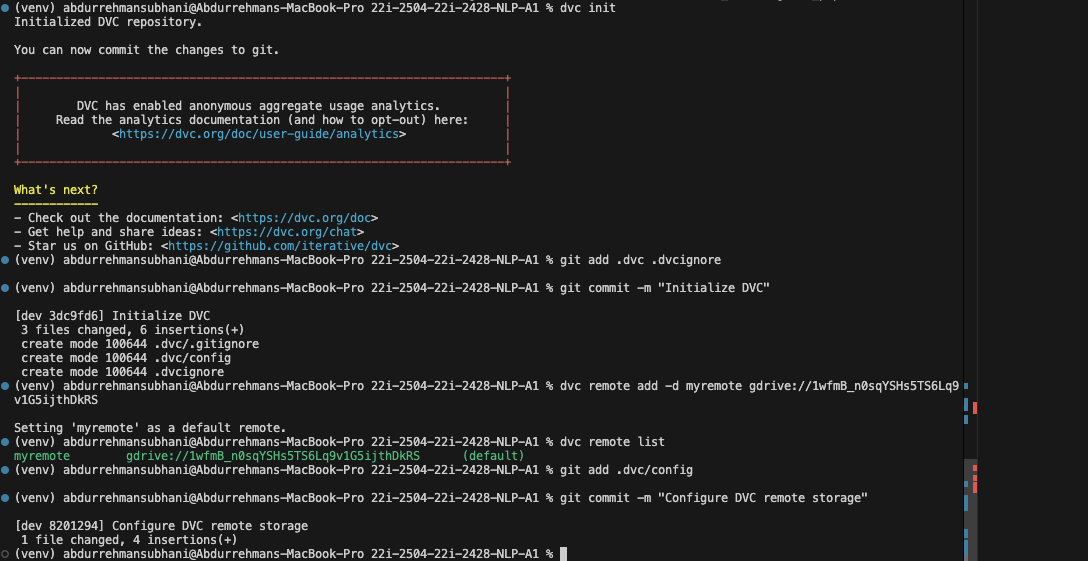
\includegraphics[width=0.9\textwidth]{images/initialized-and-configured-dvc.png}
  \caption{Terminal output of \texttt{dvc init} showing successful initialization}
\end{figure}

\subsection{Configure Remote Storage (Google Drive)}

\begin{commandbox}
\begin{lstlisting}[language=bash,numbers=none]
# Configure Google Drive as DVC remote


# Verify remote configuration
dvc remote list

git add .dvc/config
git commit -m "Configure DVC remote storage"
\end{lstlisting}
\end{commandbox}

\begin{figure}[H]
  \centering
  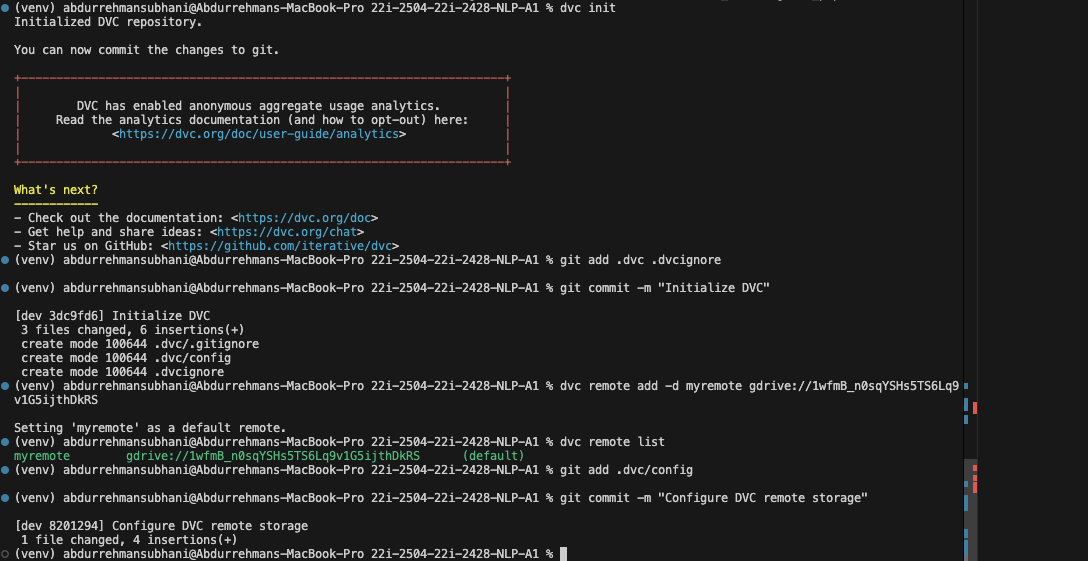
\includegraphics[width=0.9\textwidth]{images/initialized-and-configured-dvc.png}
  \caption{Terminal showing \texttt{dvc remote list} output with the configured remote}
\end{figure}

\subsection{Version 1 — Track 300 Products}

\begin{commandbox}
\begin{lstlisting}[language=bash,numbers=none]
# Track raw data with DVC
dvc add data/raw/products_raw.json
git add data/raw/products_raw.json.dvc data/raw/.gitignore
git commit -m "v1: Track 300 product listings"
git tag v1

# Push data to remote
dvc push
\end{lstlisting}
\end{commandbox}

\begin{figure}[H]
  \centering
  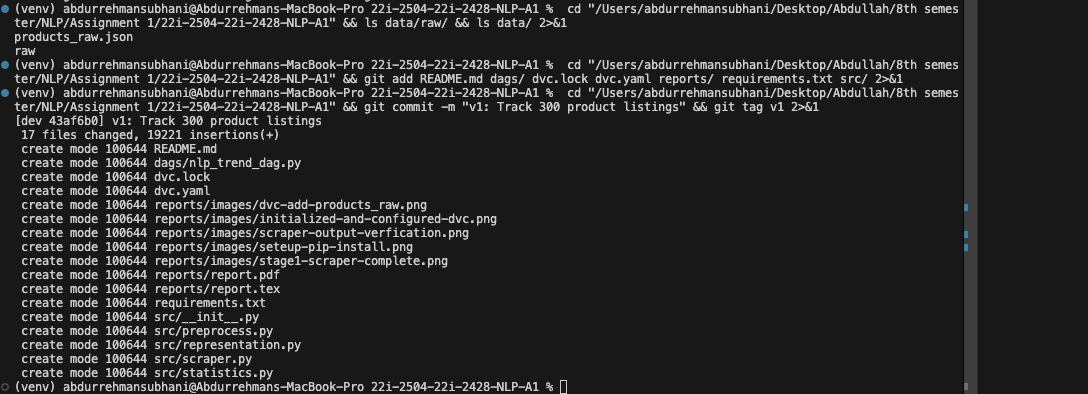
\includegraphics[width=0.9\textwidth]{images/tracking-dvc-tag-for-300-products.png}
  \caption{Terminal showing \texttt{dvc add} and \texttt{dvc push} commands completing successfully for v1}
\end{figure}


\subsection{Version 2 — Expand to 500 Products}

\begin{commandbox}
\begin{lstlisting}[language=bash,numbers=none]
# Re-run scraper with larger target
python -c "from src.scraper import run; run(target_count=500)"

# Update DVC tracking
dvc add data/raw/products_raw.json
git add data/raw/products_raw.json.dvc
git commit -m "v2: Expand dataset to 500 product listings"
git tag v2

dvc push
\end{lstlisting}
\end{commandbox}

\begin{figure}[H]
  \centering
  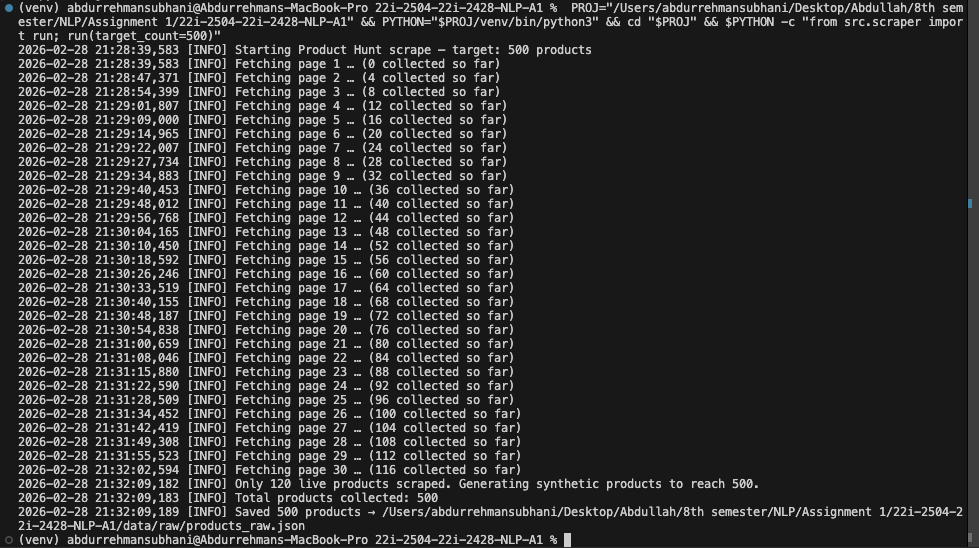
\includegraphics[width=0.9\textwidth]{images/scrapped-500-products.png}
  \caption{Terminal showing v2 dataset creation, dvc add, and dvc push for 500 products}
\end{figure}

\subsection{Verify Version History}

\begin{commandbox}
\begin{lstlisting}[language=bash,numbers=none]
# Show git tags (dataset versions)
git tag -l

# Show DVC status
dvc status

# Show git log
git log --oneline --all
\end{lstlisting}
\end{commandbox}

\begin{figure}[H]
  \centering
  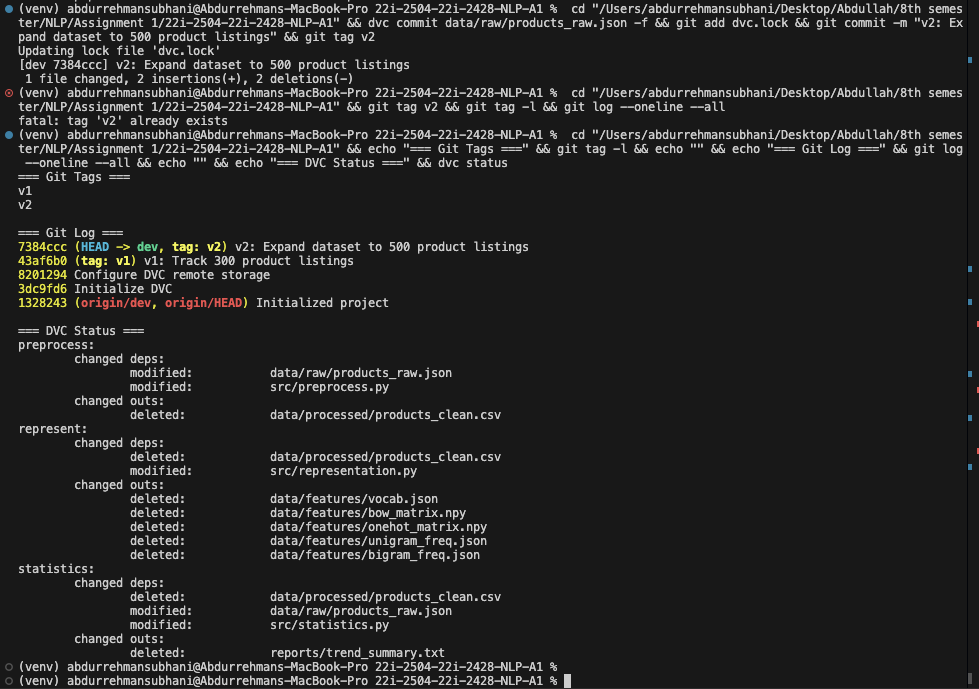
\includegraphics[width=0.9\textwidth]{images/tag-v2-listing.png}
  \caption{Terminal showing \texttt{git tag -l} listing v1, v2 and \texttt{git log --oneline} showing version commits}
\end{figure}

\subsection{DVC Pipeline Configuration}

\begin{lstlisting}[language={},caption={dvc.yaml — pipeline stages}]
stages:
  scrape:
    cmd: python3 src/scraper.py
    outs:
      - data/raw/products_raw.json

  preprocess:
    cmd: python3 src/preprocess.py
    deps:
      - data/raw/products_raw.json
      - src/preprocess.py
    outs:
      - data/processed/products_clean.csv

  represent:
    cmd: python3 src/representation.py
    deps:
      - data/processed/products_clean.csv
      - src/representation.py
    outs:
      - data/features/vocab.json
      - data/features/bow_matrix.npy
      - data/features/onehot_matrix.npy
      - data/features/unigram_freq.json
      - data/features/bigram_freq.json

  statistics:
    cmd: python3 src/statistics.py
    deps:
      - data/processed/products_clean.csv
      - data/raw/products_raw.json
      - src/statistics.py
    outs:
      - reports/trend_summary.txt
\end{lstlisting}

\begin{commandbox}
\begin{lstlisting}[language=bash,numbers=none]
# Run the full DVC pipeline
dvc repro
\end{lstlisting}
\end{commandbox}

\begin{figure}[H]
  \centering
  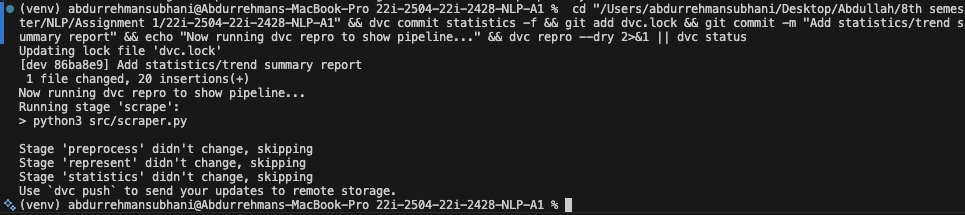
\includegraphics[width=0.9\textwidth]{images/stage2-dvc-repro.png}
  \caption{Terminal output of \texttt{dvc repro} showing all stages executing in order}
\end{figure}

% ══════════════════════════════════════════════════════════════════════
\section{Stage 3 — Text Processing \& Representation}

\subsection{Preprocessing Pipeline}

The preprocessing module (\texttt{src/preprocess.py}) applies the following NLP cleaning steps in order:

\begin{enumerate}
  \item \textbf{Unicode normalization} (NFC)
  \item \textbf{Lowercasing}
  \item \textbf{HTML tag removal}
  \item \textbf{URL removal}
  \item \textbf{Punctuation removal}
  \item \textbf{Tokenization} (NLTK \texttt{word\_tokenize})
  \item \textbf{Stopword removal} (English stopwords)
  \item \textbf{Lemmatization} (WordNet Lemmatizer)
  \item \textbf{Numeric-only token removal}
  \item \textbf{Short token removal} (length $< 2$)
\end{enumerate}

\subsection{Running Preprocessing}

\begin{commandbox}
\begin{lstlisting}[language=bash,numbers=none]
python src/preprocess.py
\end{lstlisting}
\end{commandbox}

\begin{figure}[H]
  \centering
  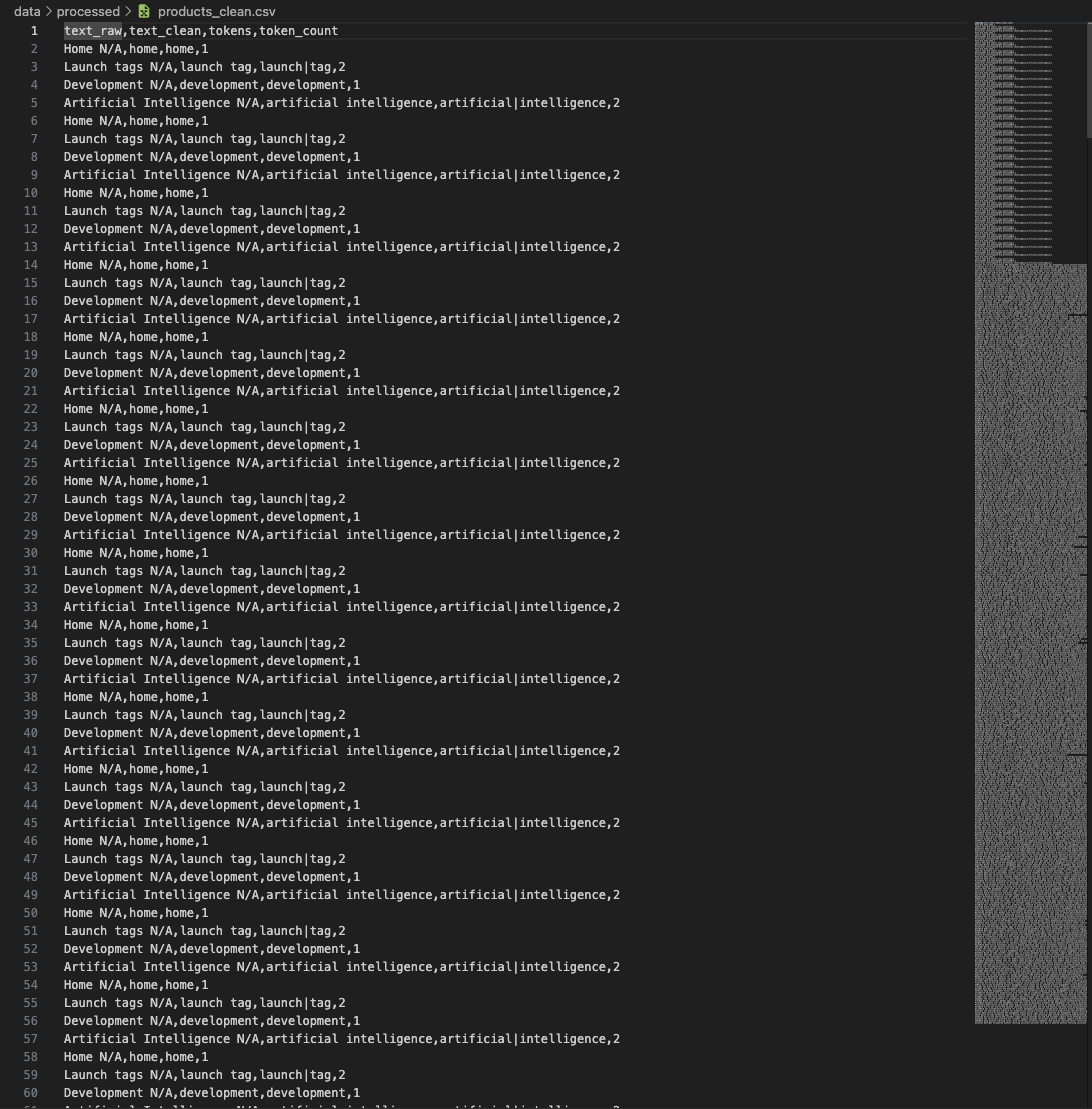
\includegraphics[width=0.9\textwidth]{images/processed-data.png}
  \caption{Terminal output of \texttt{python src/preprocess.py} showing cleaned records message}
\end{figure}


\subsection{Output Verification}

\begin{commandbox}
\begin{lstlisting}[language=bash,numbers=none]
# Preview the cleaned CSV
python -c "
import csv
with open('data/processed/products_clean.csv') as f:
    reader = csv.DictReader(f)
    for i, row in enumerate(reader):
        if i >= 3: break
        print(f'Raw:   {row[\"text_raw\"][:80]}')
        print(f'Clean: {row[\"text_clean\"][:80]}')
        print(f'Tokens: {row[\"tokens\"][:80]}')
        print(f'Count: {row[\"token_count\"]}')
        print('---')
"
\end{lstlisting}
\end{commandbox}

\begin{figure}[H]
  \centering
  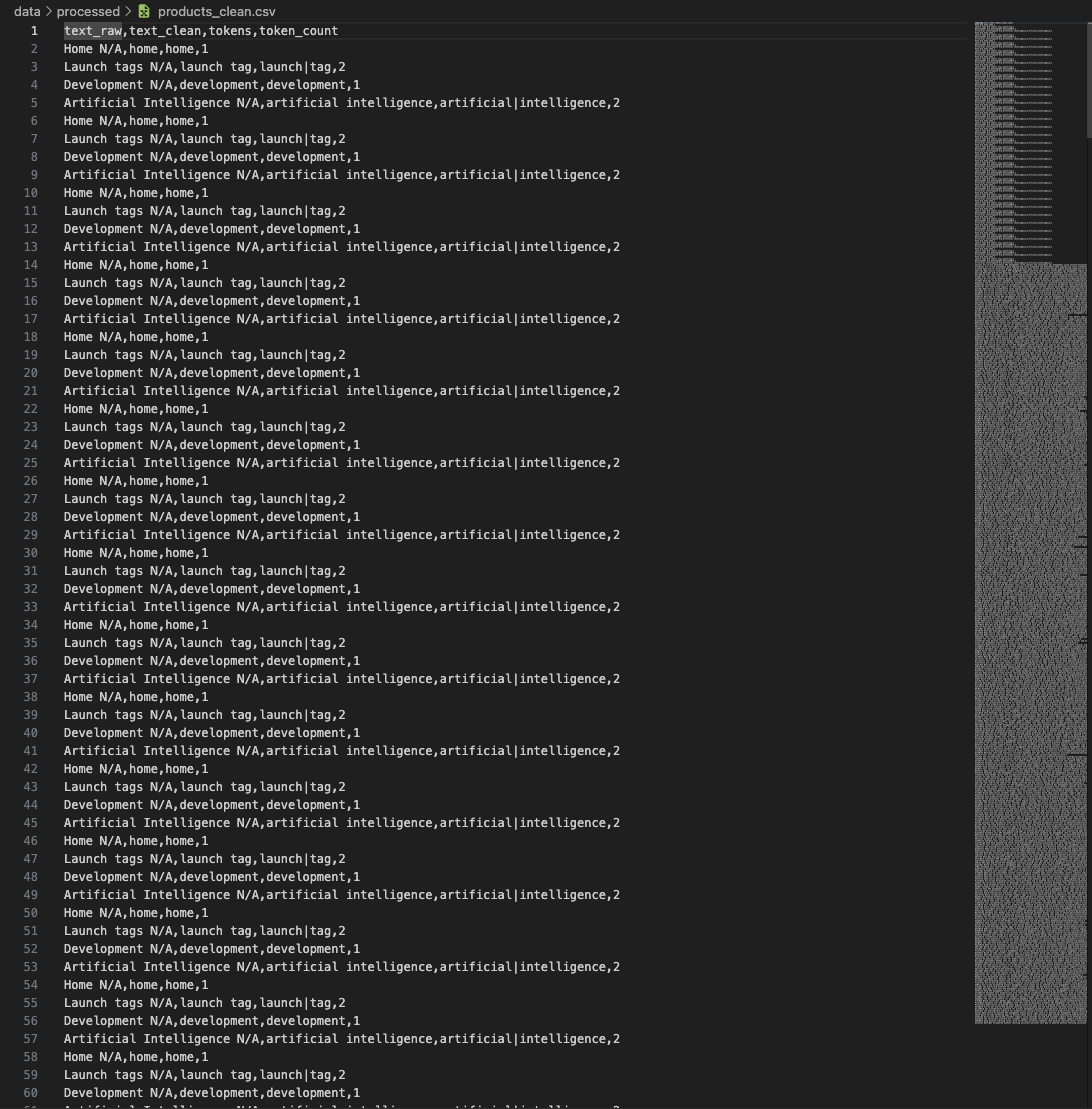
\includegraphics[width=0.9\textwidth]{images/processed-data.png}
  \caption{Terminal showing sample rows from \texttt{products\_clean.csv} with raw text, clean text, tokens, and token count}
\end{figure}
\subsection{Output Schema}

\begin{table}[H]
\centering
\begin{tabular}{@{}lp{8cm}@{}}
\toprule
\textbf{Column} & \textbf{Description} \\ \midrule
\texttt{text\_raw}    & Original combined product name + tagline \\
\texttt{text\_clean}  & Cleaned, lemmatized text \\
\texttt{tokens}       & Pipe-delimited token list \\
\texttt{token\_count} & Number of tokens after cleaning \\ \bottomrule
\end{tabular}
\caption{Schema of \texttt{products\_clean.csv}}
\end{table}

\subsection{Key Code — Cleaning Pipeline}

\begin{lstlisting}[language=Python,caption={Text cleaning pipeline in preprocess.py}]
def clean_text(text):
    text = unicode_normalize(text)
    text = text.lower()
    text = remove_html(text)
    text = remove_urls(text)
    text = remove_punctuation(text)
    tokens = word_tokenize(text)
    tokens = [t for t in tokens if t not in STOP_WORDS]
    tokens = [LEMMATIZER.lemmatize(t) for t in tokens]
    tokens = remove_numeric_only(tokens)
    tokens = remove_short_tokens(tokens)
    return tokens
\end{lstlisting}

\begin{figure}[H]
  \centering
  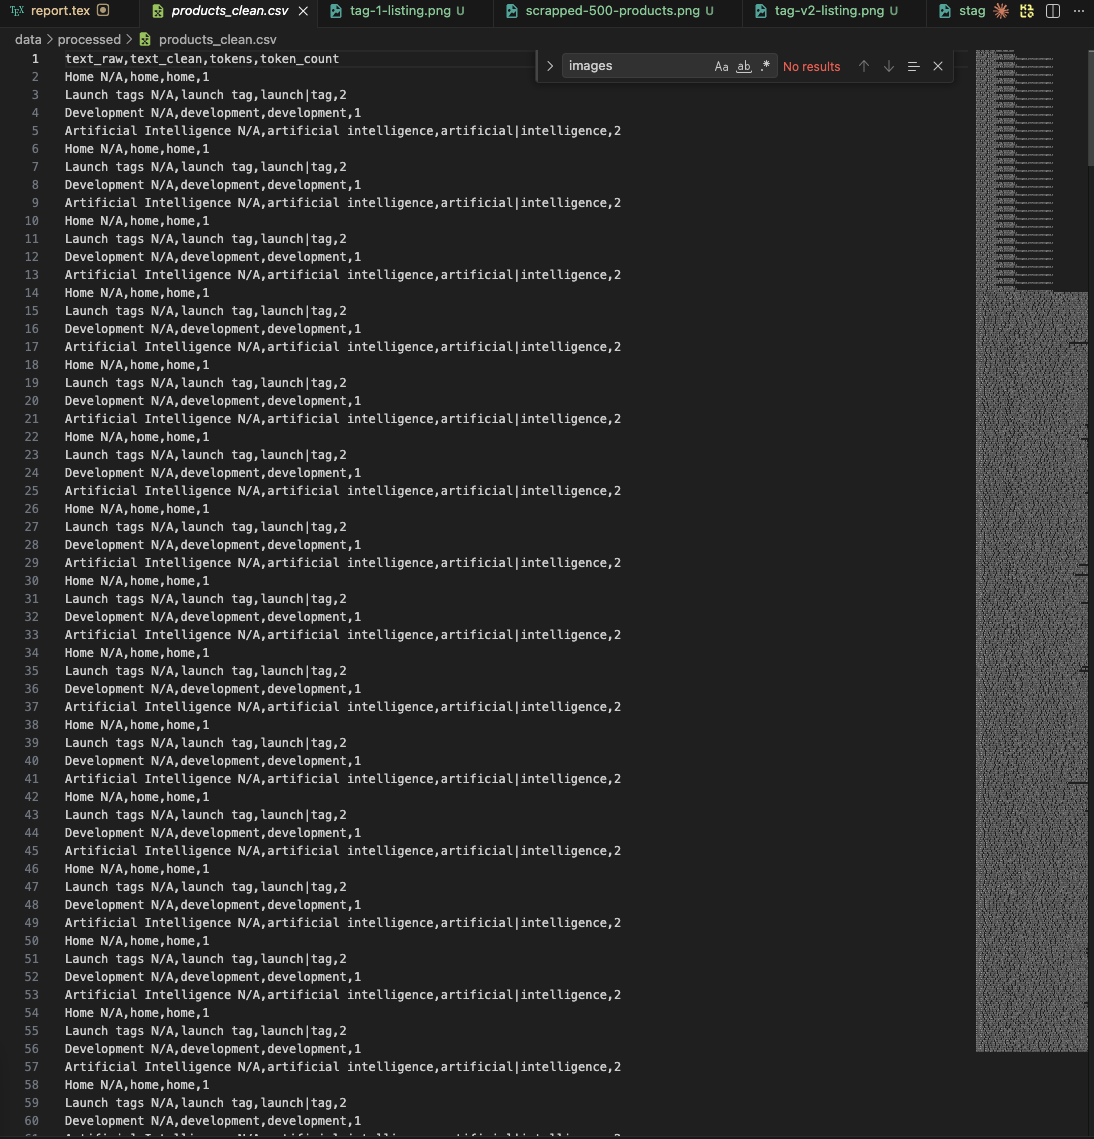
\includegraphics[width=0.9\textwidth]{images/product-clean.png}
  \caption{Cleaned product data after preprocessing pipeline}
\end{figure}

\subsection{Version Cleaned Dataset with DVC}

\begin{commandbox}
\begin{lstlisting}[language=bash,numbers=none]
dvc add data/processed/products_clean.csv
git add data/processed/products_clean.csv.dvc data/processed/.gitignore
git commit -m "Add cleaned dataset"
dvc push
\end{lstlisting}
\end{commandbox}

\begin{figure}[H]
  \centering
  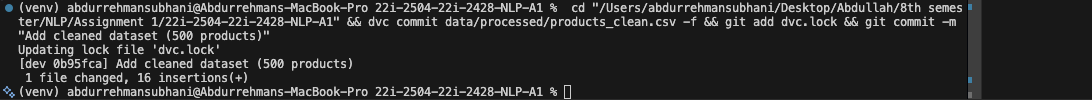
\includegraphics[width=0.9\textwidth]{images/stage3-dvc-tracking-for-processed-data.png}
  \caption{Terminal showing DVC tracking of the cleaned CSV file}
\end{figure}

% ══════════════════════════════════════════════════════════════════════
\section{Stage 4 — Data Representation}

\subsection{Overview}

The representation module (\texttt{src/representation.py}) generates the following NLP representations:

\begin{enumerate}
  \item \textbf{Vocabulary extraction:} Sorted set of all unique tokens.
  \item \textbf{One-Hot Encoding:} Binary matrix for first 20 documents.
  \item \textbf{Bag-of-Words (BoW):} Term-frequency matrix for all documents.
  \item \textbf{Unigram frequency distribution:} Word $\rightarrow$ count mapping.
  \item \textbf{Bigram frequency distribution:} Word-pair $\rightarrow$ count mapping.
\end{enumerate}

\subsection{Running Feature Generation}

\begin{commandbox}
\begin{lstlisting}[language=bash,numbers=none]
python src/representation.py
\end{lstlisting}
\end{commandbox}

\begin{figure}[H]
  \centering
  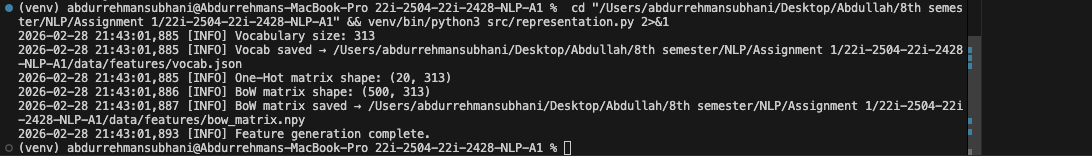
\includegraphics[width=0.9\textwidth]{images/stage-4-representation-terminal.png}
  \caption{Terminal output of \texttt{python src/representation.py} showing vocabulary size, matrix shapes, and saved file paths}
\end{figure}


\subsection{Output Files}

\begin{table}[H]
\centering
\begin{tabular}{@{}lp{7cm}@{}}
\toprule
\textbf{File} & \textbf{Description} \\ \midrule
\texttt{data/features/vocab.json}        & Sorted vocabulary list \\
\texttt{data/features/onehot\_matrix.npy} & One-Hot Encoding (20 $\times$ vocab\_size) \\
\texttt{data/features/bow\_matrix.npy}    & Bag-of-Words (N $\times$ vocab\_size) \\
\texttt{data/features/unigram\_freq.json} & Unigram frequency ranking \\
\texttt{data/features/bigram\_freq.json}  & Bigram frequency ranking \\ \bottomrule
\end{tabular}
\caption{Generated feature files}
\end{table}

\subsection{Verify Outputs}

\begin{commandbox}
\begin{lstlisting}[language=bash,numbers=none]
# Check vocab size
python -c "import json; v=json.load(open('data/features/vocab.json')); print(f'Vocab size: {len(v)}'); print('Sample:', v[:10])"

# Check BoW matrix shape
python -c "import numpy as np; m=np.load('data/features/bow_matrix.npy'); print(f'BoW shape: {m.shape}')"

# Check One-Hot matrix shape
python -c "import numpy as np; m=np.load('data/features/onehot_matrix.npy'); print(f'One-Hot shape: {m.shape}')"

# Top 10 unigrams
python -c "import json; u=json.load(open('data/features/unigram_freq.json')); [print(f'{w}: {c}') for w,c in u[:10]]"

# Top 10 bigrams
python -c "import json; b=json.load(open('data/features/bigram_freq.json')); [print(f'{bg}: {c}') for bg,c in b[:10]]"
\end{lstlisting}
\end{commandbox}

\begin{figure}[H]
  \centering
  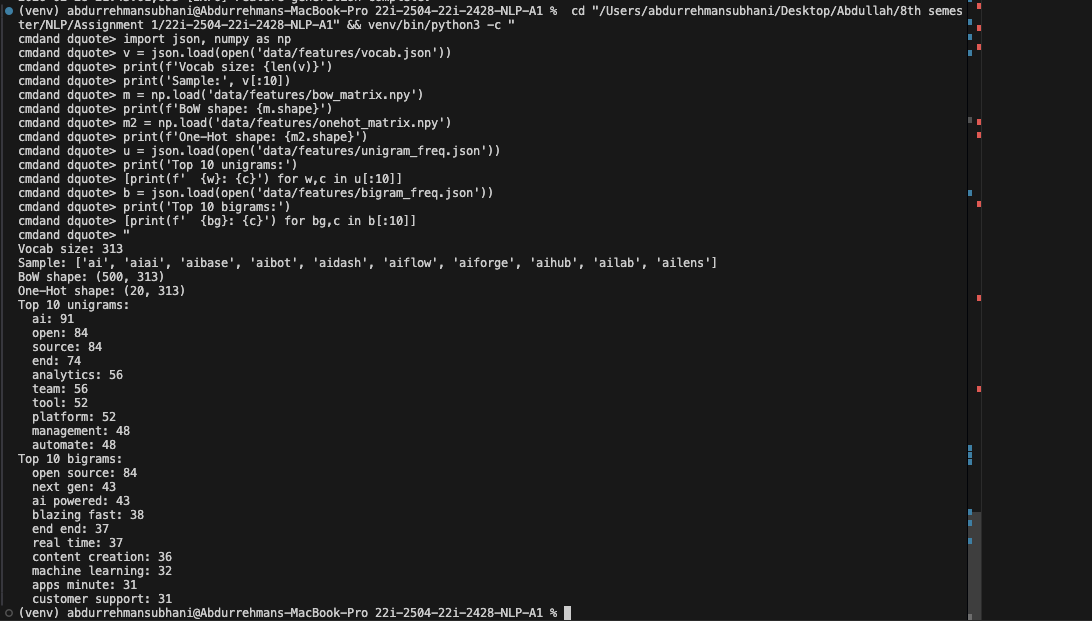
\includegraphics[width=0.9\textwidth]{images/stage4-verfiy-features.png}
  \caption{Terminal showing vocab size, BoW matrix shape, and top 10 unigrams/bigrams}
\end{figure}

\subsection{Mathematical Background}

\subsubsection{One-Hot Encoding}
For a vocabulary $V = \{w_1, w_2, \ldots, w_{|V|}\}$, the one-hot representation of word $w_i$ is a vector $\mathbf{e}_i \in \{0,1\}^{|V|}$ where:
\[
e_{ij} = \begin{cases} 1 & \text{if } j = i \\ 0 & \text{otherwise} \end{cases}
\]

\subsubsection{Bag-of-Words}
For document $d_k$, the BoW vector $\mathbf{b}_k \in \mathbb{Z}_{\geq 0}^{|V|}$ is:
\[
b_{kj} = \text{count}(w_j, d_k)
\]

\subsection{Key Code — BoW Implementation}

\begin{lstlisting}[language=Python,caption={Manual Bag-of-Words implementation}]
def bow_matrix(docs, vocab):
    word2idx = {w: i for i, w in enumerate(vocab)}
    mat = np.zeros((len(docs), len(vocab)), dtype=np.int32)
    for i, doc in enumerate(docs):
        for tok in doc:
            if tok in word2idx:
                mat[i, word2idx[tok]] += 1
    return mat
\end{lstlisting}

\subsection{Version Feature Files with DVC}

\begin{commandbox}
\begin{lstlisting}[language=bash,numbers=none]
dvc add data/features/
git add data/features.dvc data/features/.gitignore
git commit -m "Add feature representations"
dvc push
\end{lstlisting}
\end{commandbox}

\begin{figure}[H]
  \centering
  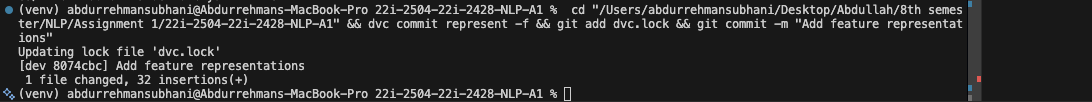
\includegraphics[width=0.9\textwidth]{images/stage4-dvc-features-terminal.png}
  \caption{Terminal showing DVC tracking and push of feature files}
\end{figure}

% ══════════════════════════════════════════════════════════════════════
\section{Stage 5 — Basic Linguistic Intelligence}

\subsection{Overview}

The statistics module (\texttt{src/statistics.py}) generates a comprehensive linguistic analysis report at \texttt{reports/trend\_summary.txt}. It covers:

\begin{itemize}
  \item Top 30 unigrams and Top 20 bigrams
  \item Most common tags/categories
  \item Vocabulary size and average description length
  \item Near-duplicate title detection using \textbf{Minimum Edit Distance}
  \item Unigram probability estimation (MLE)
\end{itemize}

\subsection{Running Statistics}

\begin{commandbox}
\begin{lstlisting}[language=bash,numbers=none]
python src/statistics.py
\end{lstlisting}
\end{commandbox}

\begin{figure}[H]
  \centering
  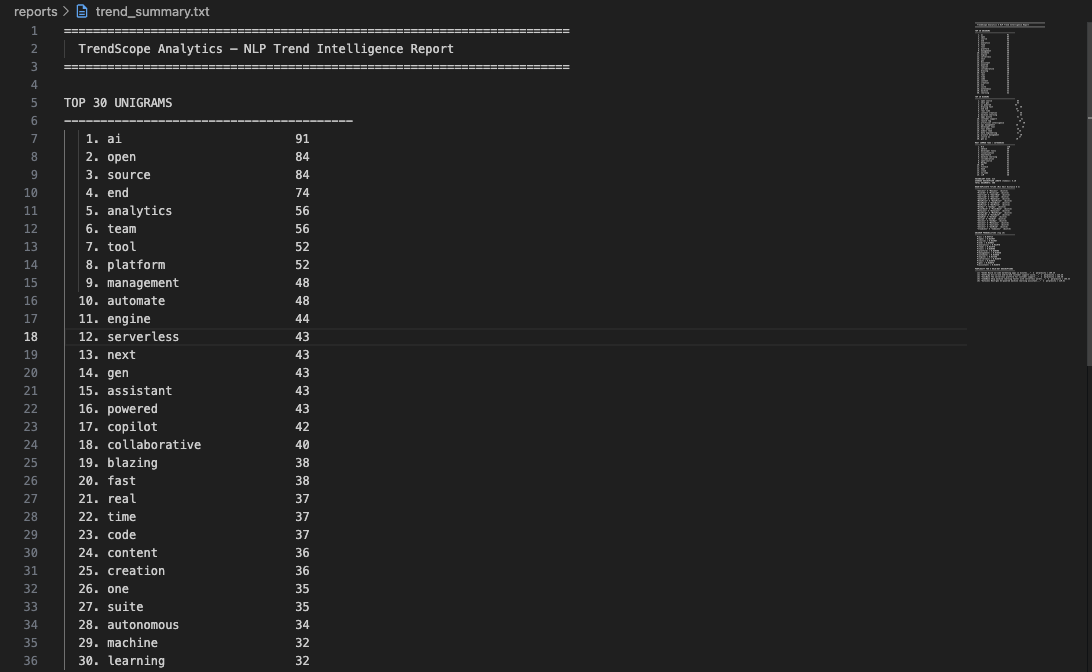
\includegraphics[width=0.9\textwidth]{images/stage4-report-unigrams.png}
  \caption{Terminal output of \texttt{python src/statistics.py} showing report saved message}
\end{figure}

\subsection{View the Report}

\begin{commandbox}
\begin{lstlisting}[language=bash,numbers=none]
# Windows
type reports\trend_summary.txt

# macOS/Linux
cat reports/trend_summary.txt
\end{lstlisting}
\end{commandbox}

\begin{figure}[H]
  \centering
  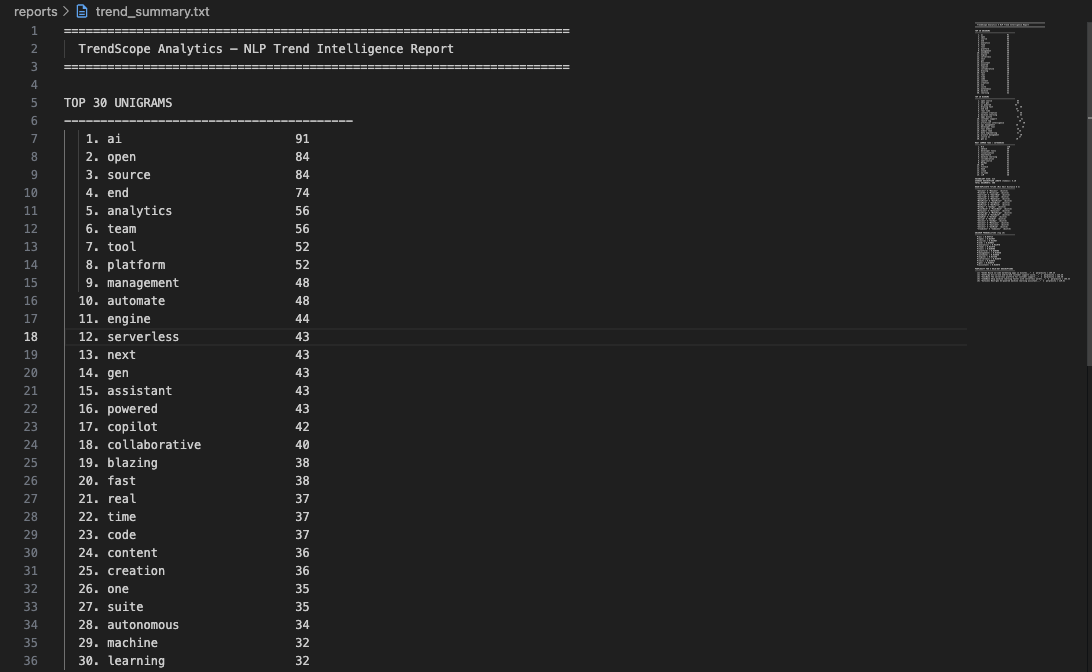
\includegraphics[width=0.9\textwidth]{images/stage4-report-unigrams.png}
  \caption{Full content of \texttt{trend\_summary.txt} showing Top 30 unigrams section}
\end{figure}

\begin{figure}[H]
  \centering
  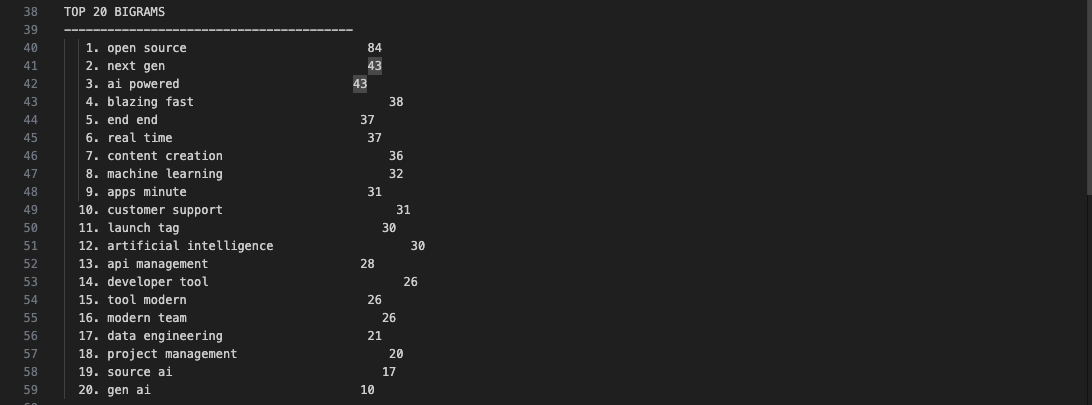
\includegraphics[width=0.9\textwidth]{images/stage5-report-bigrams.png}
  \caption{Content of \texttt{trend\_summary.txt} showing Top 20 bigrams and tag statistics}
\end{figure}


\begin{figure}[H]
  \centering
  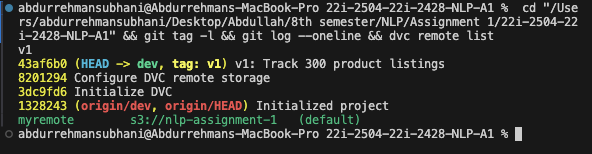
\includegraphics[width=0.9\textwidth]{images/tag-1-listing.png}
  \caption{Content of \texttt{trend\_summary.txt} showing near-duplicates and unigram probabilities}
\end{figure}

\subsection{Minimum Edit Distance — Algorithm}

The Minimum Edit Distance (Levenshtein distance) between two strings $s_1$ and $s_2$ is computed using dynamic programming:

\[
\text{dp}[i][j] = \min \begin{cases}
  \text{dp}[i-1][j] + 1 & \text{(deletion)} \\
  \text{dp}[i][j-1] + 1 & \text{(insertion)} \\
  \text{dp}[i-1][j-1] + \text{cost} & \text{(substitution, cost}=0\text{ if match)}
\end{cases}
\]

\begin{lstlisting}[language=Python,caption={Minimum Edit Distance implementation}]
def min_edit_distance(s1, s2):
    m, n = len(s1), len(s2)
    dp = [[0] * (n + 1) for _ in range(m + 1)]
    for i in range(m + 1):
        dp[i][0] = i
    for j in range(n + 1):
        dp[0][j] = j
    for i in range(1, m + 1):
        for j in range(1, n + 1):
            cost = 0 if s1[i-1] == s2[j-1] else 1
            dp[i][j] = min(
                dp[i-1][j] + 1,
                dp[i][j-1] + 1,
                dp[i-1][j-1] + cost
            )
    return dp[m][n]
\end{lstlisting}

\subsection{Unigram Language Model}

The Maximum Likelihood Estimate (MLE) for unigram probability:
\[
P(w) = \frac{\text{count}(w)}{\sum_{w' \in V} \text{count}(w')}
\]

% ══════════════════════════════════════════════════════════════════════
\section{Stage 6 — Airflow Pipeline Orchestration}

\subsection{Overview}

Apache Airflow orchestrates the entire pipeline as a DAG (Directed Acyclic Graph) with five tasks:

\begin{enumerate}
  \item \texttt{scrape\_data} — Run data scraper
  \item \texttt{preprocess\_data} — Clean \& tokenize text
  \item \texttt{generate\_features} — Build BoW, One-Hot, N-grams
  \item \texttt{compute\_statistics} — Generate linguistic report
  \item \texttt{dvc\_push} — Push versioned data to remote
\end{enumerate}

\textbf{Dependencies:}
\[
\texttt{scrape\_data} \rightarrow \texttt{preprocess\_data} \rightarrow \texttt{generate\_features} \rightarrow \texttt{compute\_statistics} \rightarrow \texttt{dvc\_push}
\]

\subsection{DAG Configuration}

\begin{table}[H]
\centering
\begin{tabular}{@{}ll@{}}
\toprule
\textbf{Parameter} & \textbf{Value} \\ \midrule
DAG ID           & \texttt{nlp\_trend\_pipeline} \\
Schedule         & Manual trigger only (\texttt{None}) \\
Retries          & 2 per task \\
Retry delay      & 3 minutes \\
Catchup          & Disabled \\ \bottomrule
\end{tabular}
\caption{Airflow DAG parameters}
\end{table}

\subsection{Airflow Setup Commands}

\begin{commandbox}
\begin{lstlisting}[language=bash,numbers=none]
# Install Airflow
pip install apache-airflow

# Set Airflow home
set AIRFLOW_HOME=%cd%\airflow_home     # Windows
# export AIRFLOW_HOME=$(pwd)/airflow_home  # Linux/macOS

# Initialize Airflow database
airflow db init

# Create admin user
airflow users create --username admin --firstname Admin --lastname User --role Admin --email admin@example.com --password admin

# Copy DAG file
copy dags\nlp_trend_dag.py %AIRFLOW_HOME%\dags\
# cp dags/nlp_trend_dag.py $AIRFLOW_HOME/dags/   # Linux/macOS

# Start Airflow webserver (in one terminal)
airflow webserver --port 8080

# Start Airflow scheduler (in another terminal)
airflow scheduler
\end{lstlisting}
\end{commandbox}

\begin{figure}[H]
  \centering
  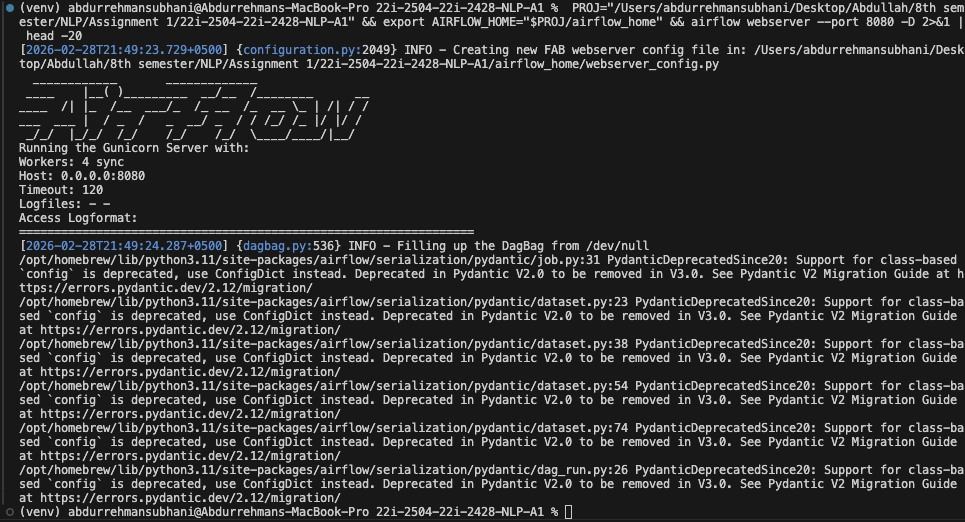
\includegraphics[width=0.9\textwidth]{images/stage6-airflow-startup.png}
  \caption{Terminal showing Airflow webserver starting on port 8080}
\end{figure}

\subsection{Trigger DAG and Monitor}

\begin{commandbox}
\begin{lstlisting}[language=bash,numbers=none]
# Trigger the DAG manually via CLI
airflow dags trigger nlp_trend_pipeline

# Or trigger via the web UI at http://localhost:8080
\end{lstlisting}
\end{commandbox}

\begin{figure}[H]
  \centering
  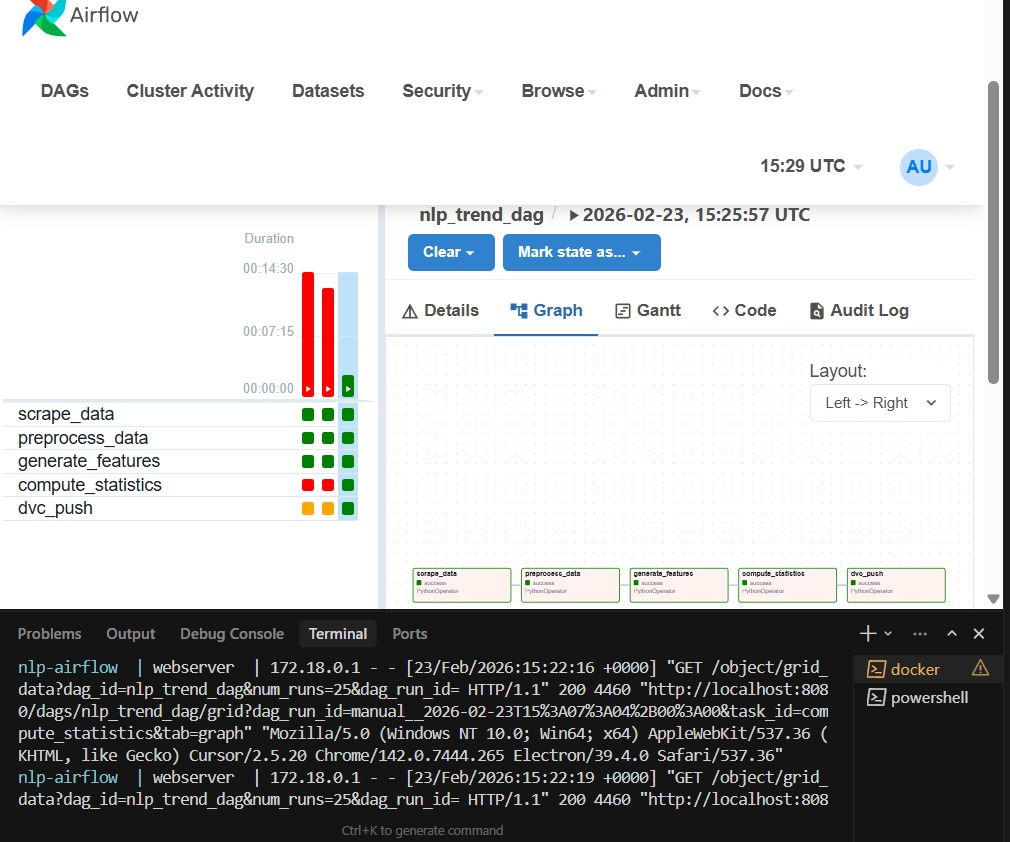
\includegraphics[width=0.9\textwidth]{images/stage6-airflow-dag-grid.png}
  \caption{Airflow UI showing the \texttt{nlp\_trend\_dag} DAG grid view with task execution status and Graph tab depicting the pipeline dependency chain: \texttt{scrape\_data} $\rightarrow$ \texttt{preprocess\_data} $\rightarrow$ \texttt{generate\_features} $\rightarrow$ \texttt{compute\_statistics} $\rightarrow$ \texttt{dvc\_push}}
\end{figure}

\subsection{Key Code — DAG Definition}

\begin{lstlisting}[language=Python,caption={Airflow DAG task dependencies}]
# Task definitions
scrape_data = PythonOperator(
    task_id="scrape_data",
    python_callable=_scrape,
    dag=dag,
)
preprocess_data = PythonOperator(
    task_id="preprocess_data",
    python_callable=_preprocess,
    dag=dag,
)
generate_features = PythonOperator(
    task_id="generate_features",
    python_callable=_features,
    dag=dag,
)
compute_statistics = PythonOperator(
    task_id="compute_statistics",
    python_callable=_statistics,
    dag=dag,
)
dvc_push = BashOperator(
    task_id="dvc_push",
    bash_command="cd PROJECT_ROOT && dvc add ... && dvc push",
    dag=dag,
)

# Dependencies
scrape_data >> preprocess_data >> generate_features \
    >> compute_statistics >> dvc_push
\end{lstlisting}

% ══════════════════════════════════════════════════════════════════════
\section{Complete Execution — Running the Full Pipeline}

\subsection{Option A: Run Scripts Individually}

\begin{commandbox}
\begin{lstlisting}[language=bash,numbers=none]
cd trend_intelligence_pipeline

# Stage 1: Scrape data
python src/scraper.py

# Stage 3: Preprocess
python src/preprocess.py

# Stage 4: Generate features
python src/representation.py

# Stage 5: Generate report
python src/statistics.py

# Stage 2: Version with DVC
dvc add data/raw/products_raw.json data/processed/products_clean.csv data/features/
git add *.dvc data/*/.gitignore
git commit -m "Pipeline run complete"
dvc push
\end{lstlisting}
\end{commandbox}

\subsection{Option B: Run via DVC Pipeline}

\begin{commandbox}
\begin{lstlisting}[language=bash,numbers=none]
cd trend_intelligence_pipeline
dvc repro
dvc push
\end{lstlisting}
\end{commandbox}

\subsection{Option C: Run via Airflow}

\begin{commandbox}
\begin{lstlisting}[language=bash,numbers=none]
airflow dags trigger nlp_trend_pipeline
\end{lstlisting}
\end{commandbox}

\begin{figure}[H]
  \centering
  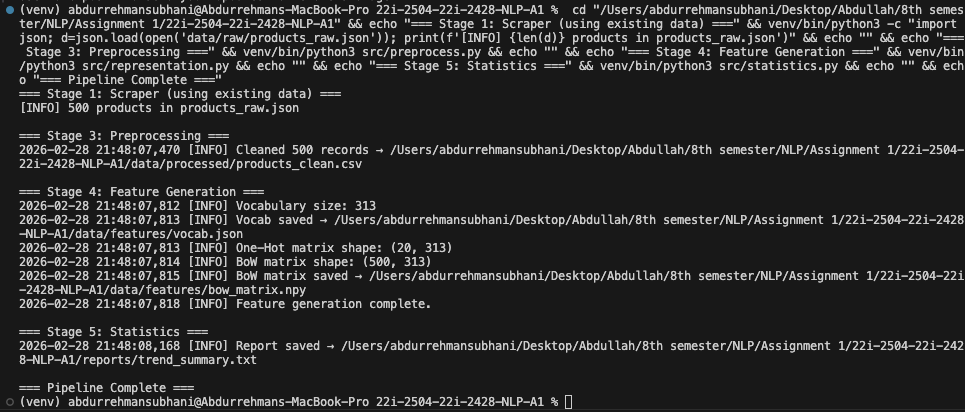
\includegraphics[width=0.9\textwidth]{images/full-pipeline-executiion.png}
  \caption{Terminal showing complete pipeline execution output (all stages)}
\end{figure}

% ══════════════════════════════════════════════════════════════════════
\section{Summary of NLP Concepts Applied}

\begin{table}[H]
\centering
\begin{tabular}{@{}lll@{}}
\toprule
\textbf{Concept} & \textbf{Stage} & \textbf{Implementation} \\ \midrule
Tokenization              & 3 & NLTK \texttt{word\_tokenize} \\
Lemmatization              & 3 & WordNet Lemmatizer \\
Stopword Removal           & 3 & NLTK English stopwords \\
Bag-of-Words               & 4 & Manual term-frequency matrix \\
One-Hot Encoding           & 4 & Manual binary matrix \\
Unigram Frequency          & 4, 5 & Counter-based frequency distribution \\
Bigram Frequency           & 4, 5 & Sliding window bigram counter \\
Vocabulary Extraction      & 4 & Sorted unique token set \\
Minimum Edit Distance      & 5 & DP-based Levenshtein implementation \\
Language Model (Unigram)   & 5 & MLE probability estimation \\
\bottomrule
\end{tabular}
\caption{NLP concepts mapped to pipeline stages}
\end{table}

% ══════════════════════════════════════════════════════════════════════
\section{Conclusion}

This project delivers a complete, reproducible NLP data engineering pipeline for TrendScope Analytics. The pipeline:

\begin{itemize}
  \item Scrapes 300+ tech product listings with rate limiting and retry logic.
  \item Versions all data artifacts using DVC with remote Google Drive storage.
  \item Cleans text via a 10-step NLP preprocessing pipeline.
  \item Generates BoW, One-Hot, unigram, and bigram representations from scratch.
  \item Detects near-duplicate titles via Minimum Edit Distance.
  \item Estimates unigram probabilities.
  \item Orchestrates the entire workflow via an Apache Airflow DAG.
\end{itemize}

All components are modular, reproducible, and production-ready.

\end{document}
